% =============================================
% 导言区
% =============================================
\documentclass{xjtureport}








% =============================================
% 正文区
% =============================================


\begin{document}

% ===导入实验报告封面==============================
\begin{titlepage}
	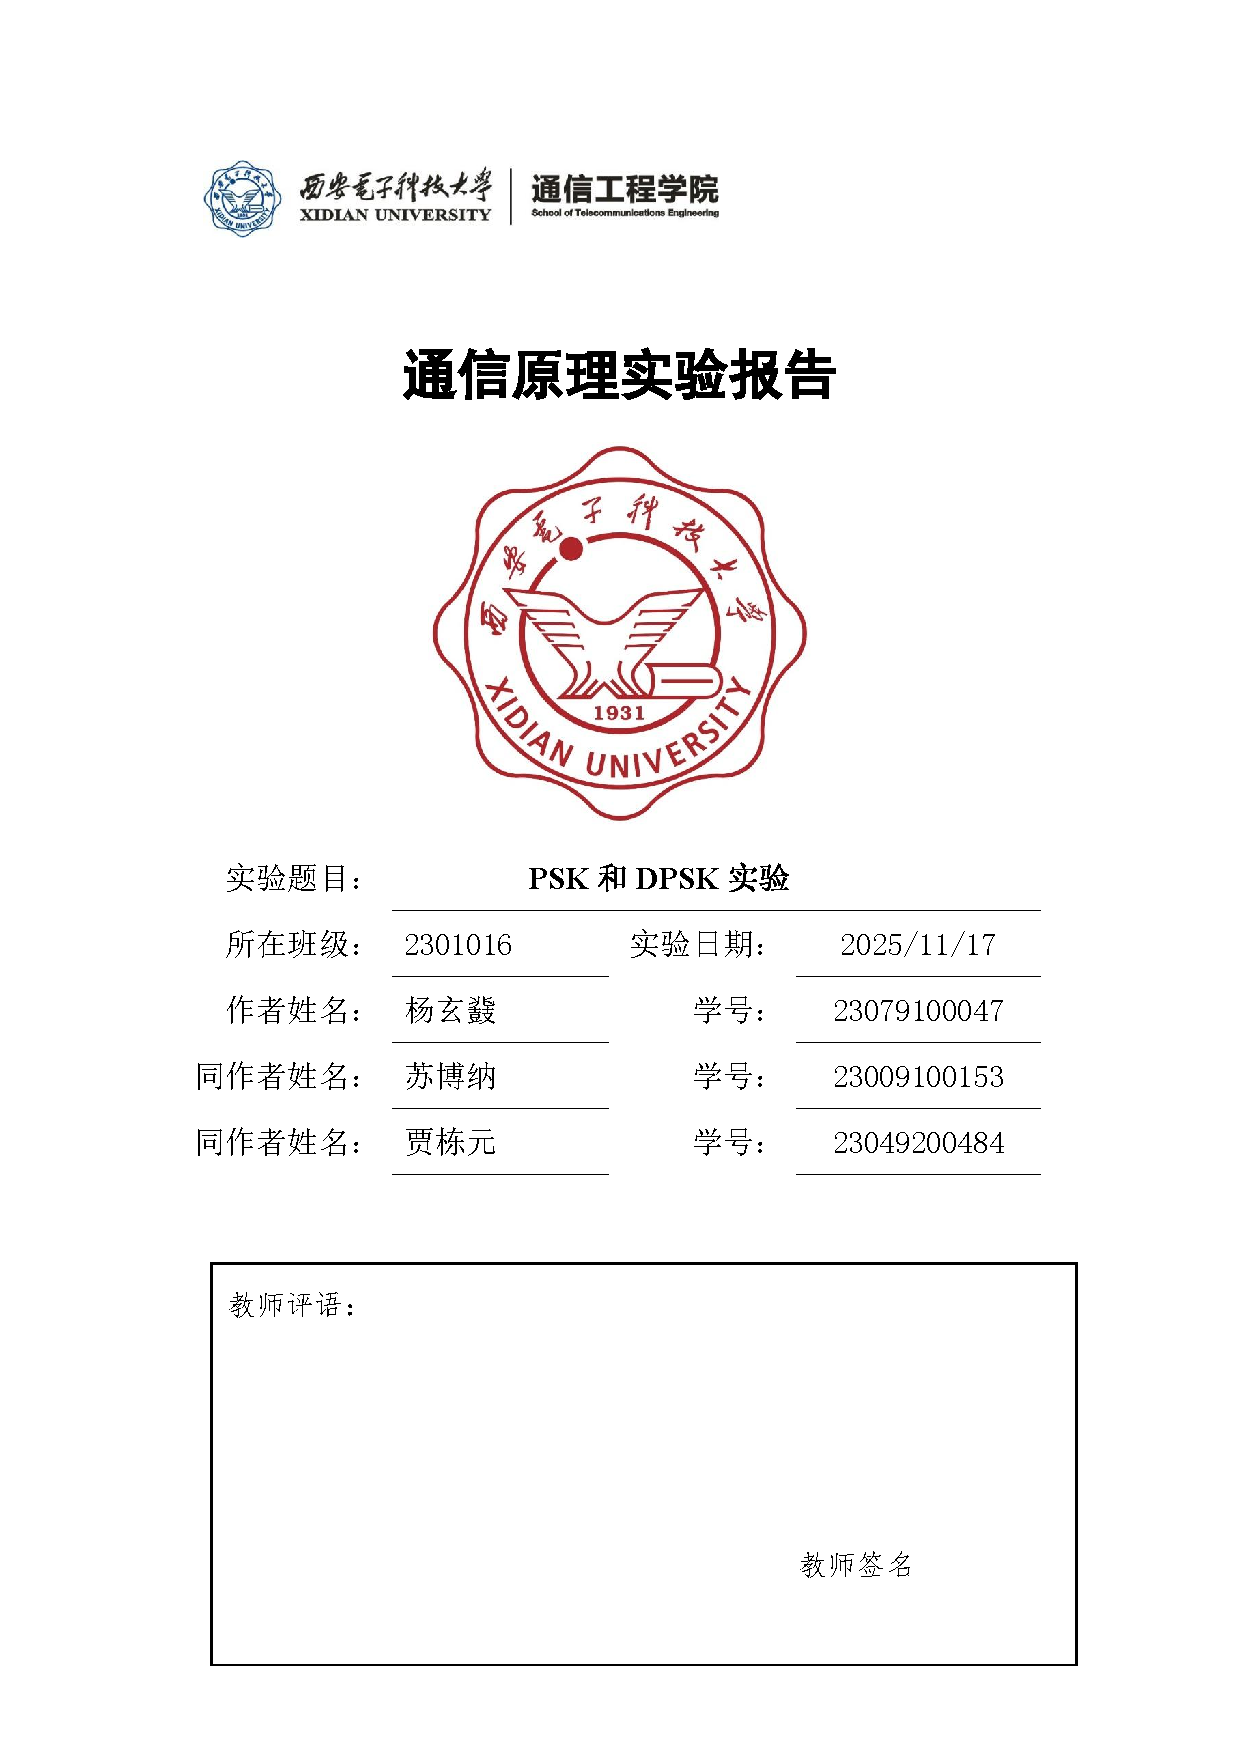
\includepdf[pages=-]{figures/实验3封面.pdf}
\end{titlepage}



% ===正文==============================


% 标题（一级居中）

\chapterinline{实验三： PSK和DPSK}

\section{实验目的}
（1）掌握 PSK 调制解调的工作原理及性能要求；

（2）进行 PSK 调制、解调实验，掌握相干解调原理和载波同步方法；

（3）理解 PSK 相位模糊的成因，思考解决办法。

（4）掌握差分编码与差分译码的原理及实现方法。

（5）掌握 DPSK 调制与解调的原理及实现方法。

（6）由“倒π”现象分析 DPSK 调制方式。

\section{实验器材}

西电通信与实验专业平台（半实物仿真）。

\section{实验内容}

\subsection*{(1)PSK调制观测}

	  \begin{enumerate}[label=\roman*.]  % 二级编号：i., ii., iii., ...
		
		\item 设置基带数据为“15-PN”，速率“64K”，观察基带信号和已调信号相位对应关系并观测记录已调信号频谱。
		
			\textbf{实验结果：}实验结果如图所示：
			
		
		\begin{figure}[H]
			\centering
			\begin{subfigure}{0.45\linewidth}
				\centering
				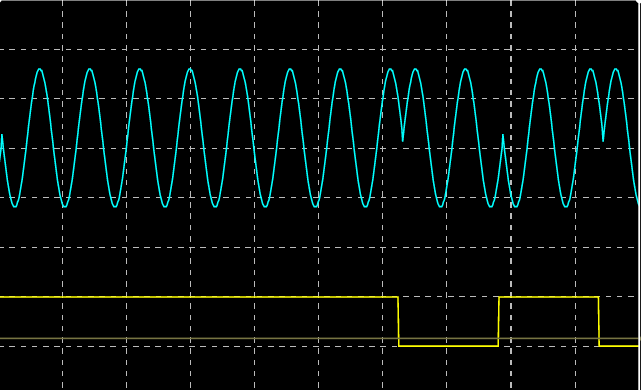
\includegraphics[width=\linewidth]{figures/基带信号与已调信号相位关系.png}
				\caption{基带与2PSK已调信号时域波形}
				\label{fig:fsk_df_gt}
			\end{subfigure}\hfill
			\begin{subfigure}{0.45\linewidth}
				\centering
				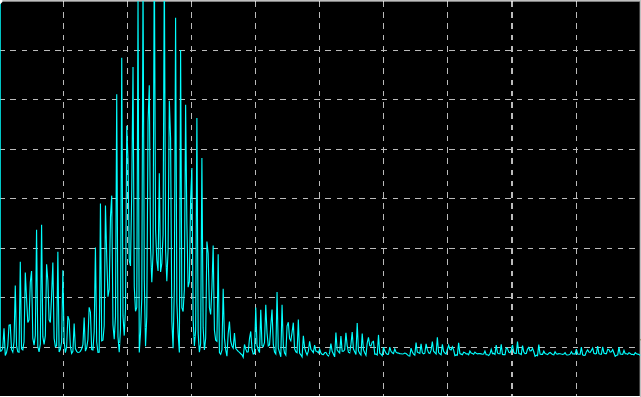
\includegraphics[width=\linewidth]{figures/已调信号频谱.png}
				\caption{2PSK已调信号频谱图}
				\label{fig:fsk_df_eq}
			\end{subfigure}
		\end{figure}
			
			\textbf{分析：}
			
			由时域波形可知，调制后载波在比特发生跳变时出现约$180^\circ$的相位翻转，而在相邻比特相同的情况下载波相位保持连续不变，符合二进制相移键控（2PSK/BPSK）的调制特性：用载波相位的两种状态（$0$和$\pi$）来分别表示二进制“1”和“0”（或反之）。
			
			从频域图像可知，调制后的信号由原基带的低频成分被“搬移”到载波频率附近，从而形成带通信号； 
			 频谱的主瓣宽度与基带码元速率成正比。
		
		\item 修改载波频率，观察记录频谱特性的变化。修改基带信号时钟速率的设置，设置为64K，128K，观测记录调制信号的频谱变化。 
		
			\textbf{基带信号时钟速率改变：}实验结果如图所示：
			
			\begin{figure}[H]
				\centering
				\begin{subfigure}{0.45\linewidth}
					\centering
					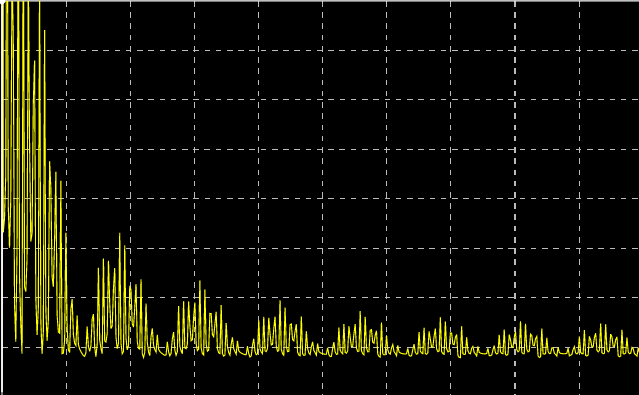
\includegraphics[width=\linewidth]{figures/调制信号频谱（载波64K）.png}
					\caption{基带码率 64K 时的 2PSK 调制信号频谱}
				\end{subfigure}\hfill
				\begin{subfigure}{0.45\linewidth}
					\centering
					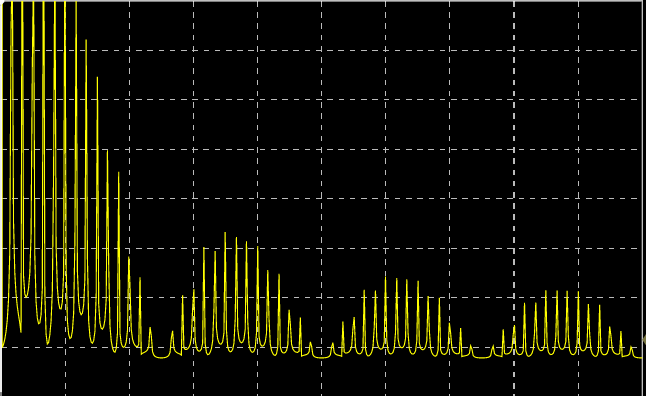
\includegraphics[width=\linewidth]{figures/调制信号频谱（载波128K）.png}
					\caption{基带码率 128K 时的 2PSK 调制信号频谱}
				\end{subfigure}
				\caption{不同基带码率下 2PSK 调制信号的频谱变化}
			\end{figure}
			
			\textbf{分析：}
			
			从实验结果可以看到，当基带码元速率从 64K 提高到 128K 时，2PSK 信号的频谱主瓣明显变宽，旁瓣间隔也随之缩小。说明 2PSK 调制信号的带宽与基带码率成正比，码率越高，频谱越宽。
			
			\textbf{载波频率改变}不同载波频率下的调制信号频谱如图所示：
			
			\begin{figure}[H]
				\centering
				\begin{subfigure}{0.45\linewidth}
					\centering
					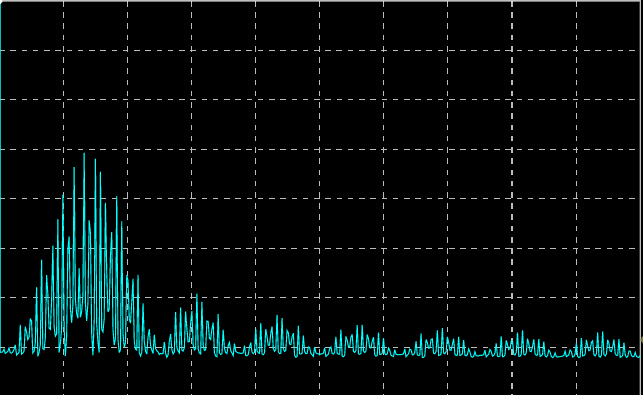
\includegraphics[width=\linewidth]{figures/已调信号频谱（载波64K）.png}
					\caption{载波频率 64K 时的 2PSK 调制信号频谱}
				\end{subfigure}\hfill
				\begin{subfigure}{0.45\linewidth}
					\centering
					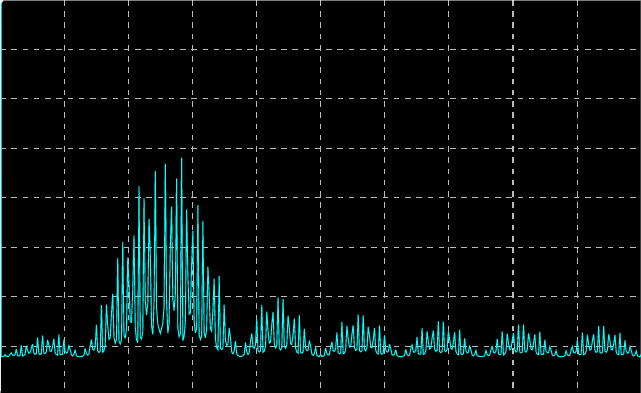
\includegraphics[width=\linewidth]{figures/已调信号频谱（载波128K）.png}
					\caption{载波频率 128K 时的 2PSK 调制信号频谱}
				\end{subfigure}
				\caption{不同载波频率下 2PSK 调制信号的频谱变化}
			\end{figure}
			
			\textbf{分析：}
			
			实验结果表明：改变载波频率时，2PSK 信号的频谱形状（主瓣宽度及旁瓣结构）基本不变，仅在频率轴上整体平移。说明载波频率只决定频谱中心位置，不影响调制信号带宽。
			
		
		\item 数据分析：
		
		\begin{enumerate}[label=\alph*)]
			\item 经 PSK 调制后，频谱有哪些变化？
			
			\textbf{答：}
			基带信号原本集中在低频附近，其频谱经过 PSK 调制后被整体搬移到载波频率附近，形成以载波为中心的带通信号。频谱出现明显的主瓣及若干旁瓣，主瓣宽度由基带码率决定，而载波的加入使频谱在高频处对称展开。
			
			\item 分析 PSK 已调信号的带宽与基带信号速率、载波频率有什么关系？
			
			\textbf{答：}
			PSK 调制信号的带宽主要由基带码元速率决定：基带速率越高，每比特持续时间越短，其频谱越宽，因此调制后的主瓣宽度也随之成比例增大。载波频率则只决定频谱在频率轴上的中心位置，不改变带宽大小。当载波提高时，整个频谱等距离向高频方向平移，其形状与宽度保持不变。
		\end{enumerate}
	
		
		\end{enumerate}
		
\subsection*{(2)PSK解调观测}

\begin{enumerate}[label=\roman*.]  % 二级编号：i., ii., iii., ...
	\item PSK相位模糊观察：利用系统中提供的修改载波相位的功能，通过框图中“VCO”按钮，观察正常状态和相位模糊状态。
	
	\textbf{实验结果：}实验结果如图所示：
	
	\begin{figure}[H]
		\centering
		\begin{subfigure}{0.45\linewidth}
			\centering
			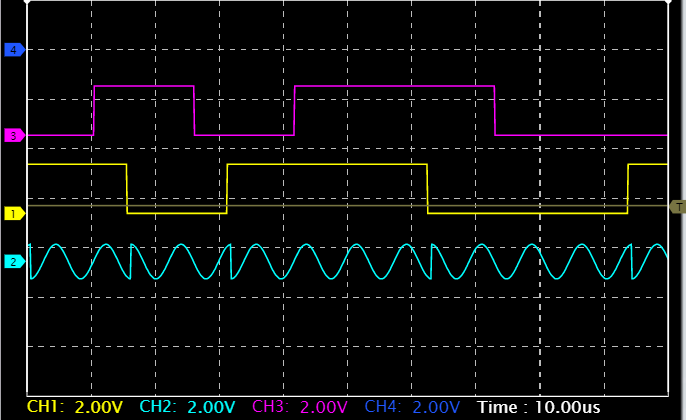
\includegraphics[width=\linewidth]{figures/相位模糊观测（正常）.png}
			\caption{正常相位锁定状态（解调数据与原基带一致）}
		\end{subfigure}\hfill
		\begin{subfigure}{0.45\linewidth}
			\centering
			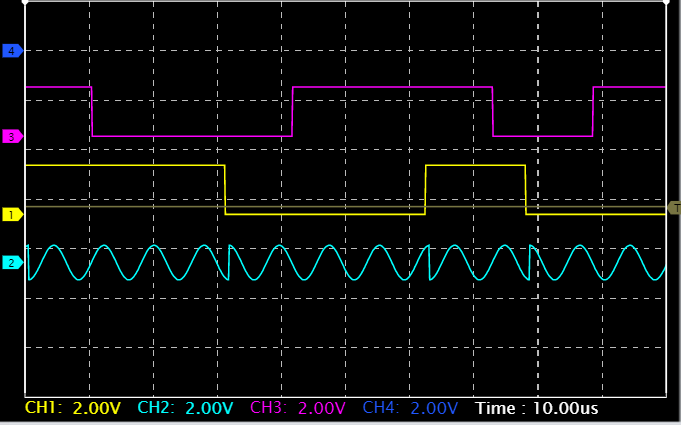
\includegraphics[width=\linewidth]{figures/相位模糊观测（反相）.png}
			\caption{相位模糊状态（解调数据整体翻转）}
		\end{subfigure}
		\caption{PSK 解调中正常状态与相位模糊状态的对比}
	\end{figure}
	
	\textbf{分析：}
	
	从图中可以看到，在正常状态下，解调输出数据与原基带 PN 序列保持一致；当本地载波相位反转 $180^\circ$ 后，解调输出的比特序列整体翻转，即所有“1”变成“0”，“0”变成“1”。
	
	说明 PSK 在相干解调中存在 \textbf{相位模糊}：由于 BPSK 信号仅包含 $0$ 和 $\pi$ 两种相位，本地载波若与输入信号相差$180^\circ$，仍能成功锁定，但输出数据将整体反相。相位模糊不影响频谱与锁相状态，但会导致解调比特出现整体符号翻转。
	
	
	\item 分析和回答：
	
	\begin{enumerate}[label=\alph*)]
		\item 什么是相位模糊？
		
		\textbf{答：}
		PSK 解调时如果本地载波和调制信号载波反相，则输出的基带数据也会反相，这就是相位模糊。
		
		\item 相位模糊如何克服？
		
		\textbf{答：}
		相位模糊可通过在调制中加入唯一确定相位的附加信息来消除，常用方法包括：
		\begin{itemize}
			\item 采用 \textbf{差分编码（DPSK）}：信息通过相邻比特的相位差表示，整体相位翻转不会影响解调。
			\item 使用 \textbf{已知同步序列或导频}，在接收端通过比对确定正确的相位极性。
			\item 在系统协议层加入帧头、CRC 等结构，通过判断数据是否反相来恢复正确符号。
		\end{itemize}
		其中差分编码（2DPSK）是最常用且硬件实现最简单的解决方法。
	\end{enumerate}
	
\end{enumerate}


\subsection*{(3) 噪声对 PSK 信道影响}

\textbf{实验结果：}

\begin{table}[H]
	\centering
	\begin{tabular}{|c|c|c|c|c|c|}
		\hline
		序号 & 基带速率 & 载波频率 & 载波幅度(Vpp) & 出现误码时噪声幅度(Vpp) & 信噪比（dB） \\
		\hline
		1 & 8K  & 128K & 4.00V & 0.76V & 5.26 \\
		\hline
		2 & 16K & 128K & 4.00V & 0.84V & 4.76 \\
		\hline
	\end{tabular}
\end{table}

\textbf{分析：}

实验结果表明，随着基带速率从 8K 提高到 16K，出现误码所需的噪声幅度略有增加，但对应的信噪比反而下降，说明高速基带信号对噪声更加敏感。其原因在于：

\begin{itemize}
	\item 基带速率越高，比特持续时间越短，眼图张开度变小；
	\item 信号的有效带宽增大，更容易受到高频噪声的干扰；
	\item 解调窗口缩小，使判决对噪声的容忍度下降。
\end{itemize}

因此，PSK 信号在较高码率下抗噪声性能下降，需要更高的信噪比才能保证可靠通信。本实验结果与 PSK 的理论分析一致：\textbf{码率越高，抗干扰能力越弱；信噪比越低时，误码率随之升高。}


%\begin{enumerate}[label=\roman*.]  % 二级编号：i., ii., iii., ...
%	\item 
%	
%	\textbf{实验结果与分析：}
%	
%	\item 数据分析：
%	
%	\begin{enumerate}[label=\alph*)]
%		\item 
%		
%		\textbf{答：}
%		
%	\end{enumerate}
%	
%\end{enumerate}

\subsection*{(4)2DPSK}

\begin{enumerate}[label=\roman*.]  % 二级编号：i., ii., iii., ...
	\item 差分编码观测（绝对码-相对码转换）：使用鼠标点击“基带设置”按钮，设置基带数据为：“15-PN”，设置基带时钟为“128K”。使用4通道示波器通道分别观察：绝对码-2P6、对应的相对码-4VT13和2TP8，分析差分编码输出是否正确。（注：相对码数据读取时延时一个码元）将基带数据设置为：“16bit”，“128K”，自设16bit拨码开关，观察绝对码-相对码转换是否正确。
	
	\textbf{实验结果：}实验结果如图所示：
	
	\begin{figure}[H]
		\centering
		\begin{subfigure}{0.45\linewidth}
			\centering
			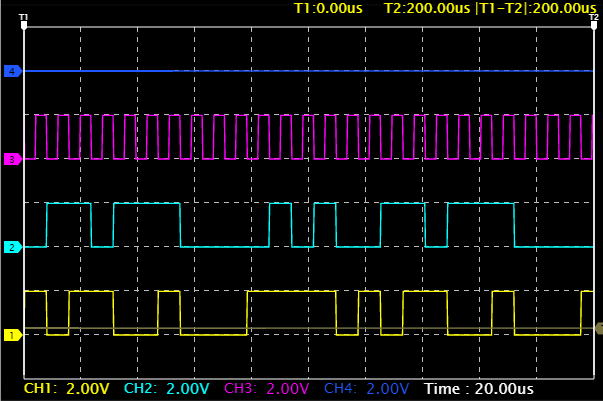
\includegraphics[width=\linewidth]{figures/绝对码相对码转换（15-PN）.png}
			\caption{15-PN 序列的绝对码与相对码转换结果}
		\end{subfigure}\hfill
		\begin{subfigure}{0.45\linewidth}
			\centering
			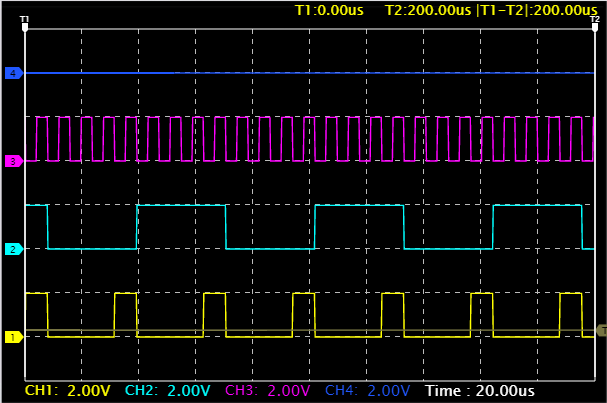
\includegraphics[width=\linewidth]{figures/绝对码相对码转换（16bit）.png}
			\caption{16bit 的绝对码与相对码转换结果}
		\end{subfigure}
		\caption{差分编码（绝对码→相对码）观测实验结果}
	\end{figure}
	
	\textbf{分析：}
	
	由图可见，相对码 4VT13 与绝对码 2P6 存在一个码元周期的延时。相对码的取值满足：当当前比特与前一比特相同，相对码输出为 0；当当前比特与前一比特不同，相对码输出为 1。
	
	从两张图（15-PN 与 16bit 拨码）均可观察到：绝对码- 相对码转换是正确的。
	
	
	\item 观察基带信号、差分输出和已调信号相位的对应关系并记录，时钟要求如 1）部分中要求。
	
	\textbf{实验结果：}
	
	实验结果如图所示：
	
	\begin{figure}[H]
		\centering
		\begin{subfigure}{0.45\linewidth}
			\centering
			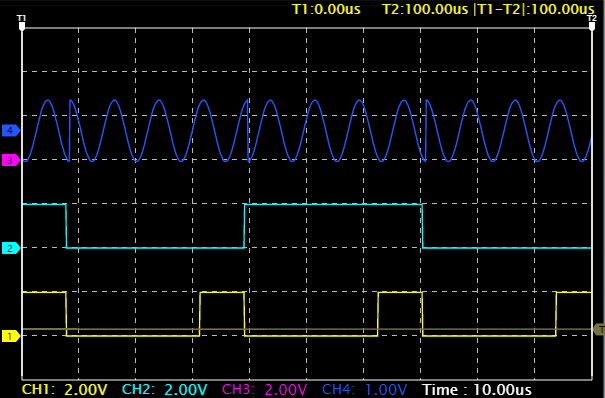
\includegraphics[width=\linewidth]{figures/基带信号_差分输出_已调信号.png}
			\caption{基带信号、差分输出与 DPSK 已调信号（示例 1）}
		\end{subfigure}\hfill
		\begin{subfigure}{0.45\linewidth}
			\centering
			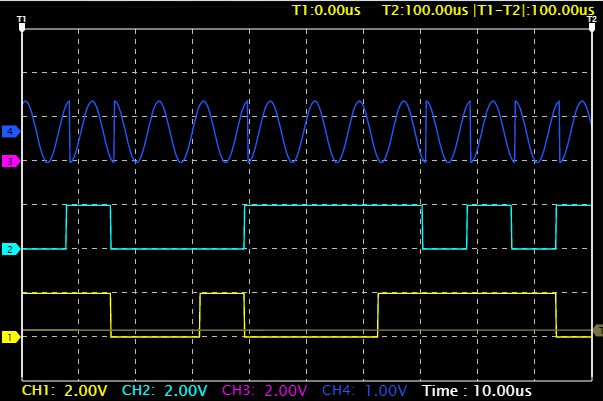
\includegraphics[width=\linewidth]{figures/基带信号_差分输出_已调信号（15-PN）.png}
			\caption{基带信号、差分输出与 DPSK 已调信号（示例 2）}
		\end{subfigure}
		\caption{DPSK 调制过程中基带、差分码与已调信号的对应关系}
	\end{figure}
	
	\textbf{分析：}
	
	从图中可观察到：基带绝对码变化后，差分输出（相对码）按异或关系产生跳变，并相对于绝对码延迟一个码元；DPSK 已调信号的相位翻转位置严格与相对码的变化一致：相对码为 1 时已调信号发生 $\pi$ 相移，相对码为 0 时相位保持不变；
	
	综上，实验结果验证了 DPSK 调制的特点：\textbf{已调信号的相位与相对码一一对应，与基带绝对码无直接关系}。
	
	
	\item 修改载波频率，观察记录频谱特性的变化。修改基带信号时钟速率的设置，设置为64K，128K，观测记录调制信号的频谱变化。
	
	\textbf{修改载波频率，实验结果：}
	
	实验中将载波频率从 256K、512K、1024K 逐步提高到 2048K，测得的 DPSK 调制信号频谱如图所示：
	
	\begin{figure}[H]
		\centering
		\begin{subfigure}{0.45\linewidth}
			\centering
			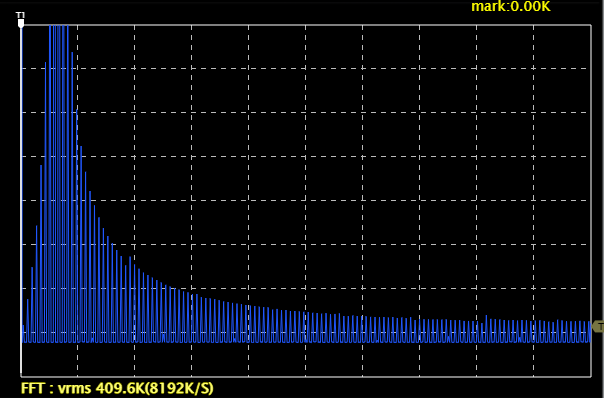
\includegraphics[width=\linewidth]{figures/DPSK已调信号频谱（载波256K）.png}
			\caption{载波频率 256K}
		\end{subfigure}\hfill
		\begin{subfigure}{0.45\linewidth}
			\centering
			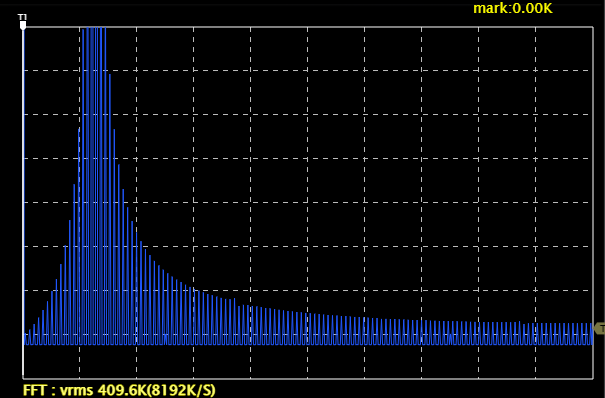
\includegraphics[width=\linewidth]{figures/DPSK已调信号频谱（载波512K）.png}
			\caption{载波频率 512K}
		\end{subfigure}
		
		\begin{subfigure}{0.45\linewidth}
			\centering
			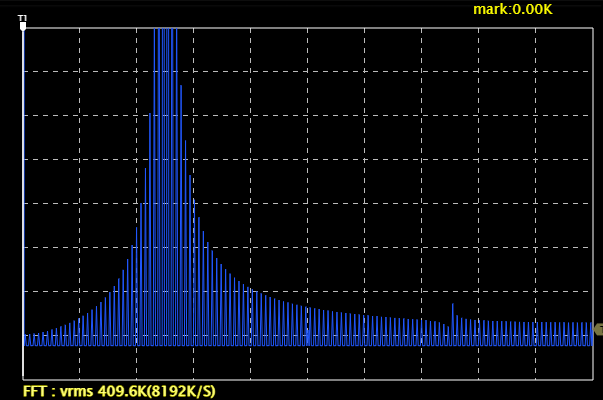
\includegraphics[width=\linewidth]{figures/DPSK已调信号频谱（载波1024K）.png}
			\caption{载波频率 1024K}
		\end{subfigure}\hfill
		\begin{subfigure}{0.45\linewidth}
			\centering
			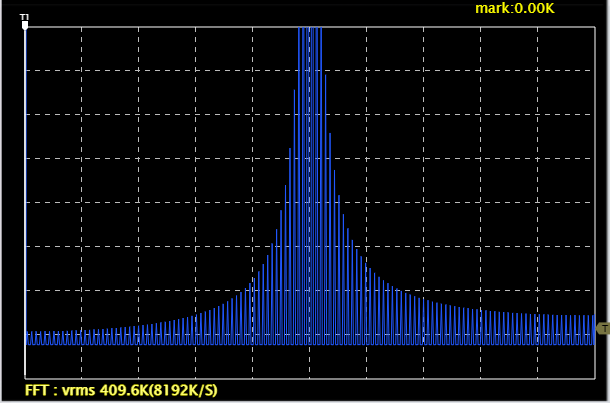
\includegraphics[width=\linewidth]{figures/DPSK已调信号频谱（载波2048K）.png}
			\caption{载波频率 2048K}
		\end{subfigure}
		
		\caption{不同载波频率下的 DPSK 已调信号频谱}
	\end{figure}
	
	\textbf{分析：}
	
	实验结果显示，随着载波频率提高，DPSK 信号的频谱形状（主瓣宽度、旁瓣结构）保持不变，仅在频率轴上整体平移。说明：载波频率只影响频谱中心位置，不改变调制信号带宽。
	
	\textbf{修改时钟频率，实验结果：}
	
	实验中将基带码率从 64K 提高到 128K，对应的 DPSK 调制信号频谱如下：
	
	\begin{figure}[H]
		\centering
		\begin{subfigure}{0.45\linewidth}
			\centering
			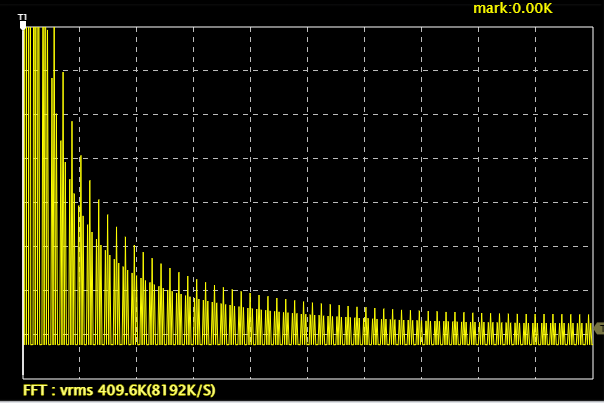
\includegraphics[width=\linewidth]{figures/DPSK调制信号频谱（时钟64K）.png}
			\caption{基带时钟 64K}
		\end{subfigure}\hfill
		\begin{subfigure}{0.45\linewidth}
			\centering
			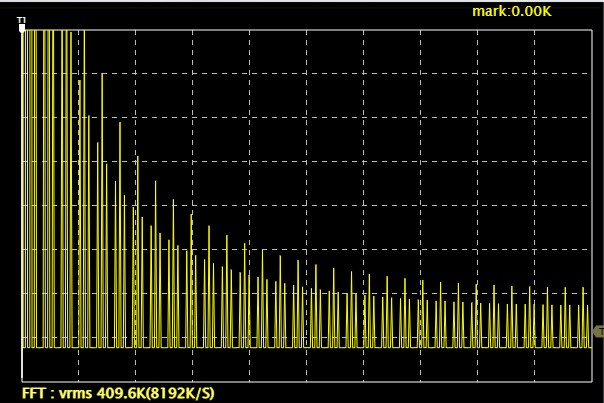
\includegraphics[width=\linewidth]{figures/DPSK调制信号频谱（时钟128K）.png}
			\caption{基带时钟 128K}
		\end{subfigure}
		\caption{不同基带码率下的 DPSK 调制信号频谱}
	\end{figure}
	
	\textbf{分析：}
	
	由图可见，基带速率从 64K 提高到 128K 后，DPSK 信号的频谱主瓣显著变宽，旁瓣间隔缩小。说明：DPSK 调制信号的带宽与基带码率成正比，码率越高，频谱越宽。
	
	\item 数据分析：
	
	\begin{enumerate}[label=\alph*)]
		\item 2DPSK是如何PSK相位模糊的？
		
		\textbf{答：}
		2DPSK 在调制前对基带信号进行差分编码，使信息由“绝对相位”改为“相邻码元之间的相位差”来表示。解调后再通过差分译码恢复原始数据。即使本地载波出现 $180^\circ$ 的相位反转（相位模糊），所有已调相位将整体翻转，但相邻符号之间的“相位差”保持不变，因此差分译码仍能得到正确的基带数据。故 2DPSK 能有效克服 PSK 的相位模糊问题。
		
		\item 2DPSK已调信号的带宽与基带信号速率、载波频率有什么关系？
		
		\textbf{答：}
		2DPSK 属于相位调制，其频谱形状与 PSK 基本相同。已调信号的带宽主要由基带码元速率决定：码率越高，频谱主瓣越宽，带宽近似与码率成正比。而载波频率仅决定频谱在频率轴上的中心位置，不影响带宽大小。因此，2DPSK 的带宽与基带速率有关，与载波频率无关。
		
		
	\end{enumerate}
	
\end{enumerate}

\section{问题回答}

\subsection*{1.在基带信号未知的情况下，能否通过已调信号波形或者频谱来区分2DPSK和PSK调制，为什么？ }

\textbf{答：}
不能。2DPSK 与普通 PSK 在已调信号的波形和频谱上具有相同的特性：两者都是利用载波相位的变化进行调制，其相位、频谱展宽规律均由基带码元速率决定，而差分编码仅对符号间的相位关系进行逻辑变换，不会改变已调信号的频谱形状，也不会在波形上产生可直接识别的特征。因此在不知道基带数据的情况下，仅凭波形或频谱无法区分是 PSK 还是 2DPSK 调制。

\section{心得体会}

通过本次实验，我对 PSK 与 DPSK 调制解调的原理和实现过程有了更加直观且深入的理解。以往在课堂上学习相位调制时，对“相位翻转”“相位模糊”等概念的认识主要依赖理论推导，而在本实验中，通过观察示波器上基带信号、相干解调信号以及差分编码后的相位变化，我能够清晰地看到各个信号之间的因果关系，从而使抽象的概念变得具体可见。

在实验过程中，我特别体会到差分编码的重要性。PSK 在解调时确实会出现 $180^\circ$ 的相位模糊，导致解调序列整体翻转，而 DPSK 通过差分方式让信息承载在“相位差”而非“绝对相位”上，从根本上解决了这一问题。通过对比相位正常和相位反转时的 2DPSK 解调输出，我更加理解了差分调制在实际通信系统中广泛应用的原因。

此外，在频谱观察部分，我认识到载波频率和基带码元速率对调制信号带宽的影响规律：载波频率只决定频谱中心的位置，而带宽主要由基带码率决定。通过改变载波和码率并对比频谱结构，我对带通信号的频域特性有了更深刻的掌握。

总体而言，本次实验不仅巩固了课堂所学的理论知识，也提升了我利用示波器分析信号、理解通信系统结构的能力。


\end{document}